\documentclass[10pt]{article}         %% What type of document you're writing.
%\documentclass[aps,prb,reprint,longbibliography]{revtex4-1}
\usepackage[letterpaper,bindingoffset=0.0in,left=1in,right=1in,top=1in,bottom=1in,footskip=.25in]{geometry}

\usepackage{amssymb}
\usepackage{color}
\usepackage{amsmath}
\usepackage{grffile}
\usepackage{cancel}
\usepackage{hyperref}
%\usepackage{calrsfs} % for \cal

% The following metadata will show up in the PDF properties
\hypersetup{
  pdfproducer= none,  % producer of the document
  pdfcreator = none,  % producer of the document
  colorlinks = true,
  allcolors = black, %-- use this if you want to set all links to the same color
}

%\usepackage{comment}
%\excludecomment{figure}
%\documentclass[aps,prb,reprint,groupedaddress]{revtex4-1}
%\linespread{1.5}
%\documentclass[aps,rmp,reprint,groupedaddress]{revtex4-1}
%\documentclass[aps,rmp,reprint,groupedaddress]{revtex4-1}
\usepackage{amssymb}
\usepackage{color}
\usepackage{amsmath}
\usepackage{epstopdf}

\usepackage{array}

\usepackage{bm}
\usepackage[english]{babel}
% You should use BibTeX and apsrev.bst for references
% Choosing a journal automatically selects the correct APS
% BibTeX style file (bst file), so only uncomment the line
% below if necessary.
%\bibliographystyle{apsrev4-1}

% include graphics with the command \includegraphics
\usepackage{graphicx}
\usepackage{tikz}
\usetikzlibrary{positioning}
\usepackage{ifthen}
\usepackage{xstring}

\usepackage[T1]{fontenc}

\usepackage[cal=cm,scrscaled=1.05]{mathalfa}

\date{\vspace{-5ex}}

\begin{document}
\newcommand{\w}{0.15}
\newcommand{\h}{0.4}
\newcommand{\hc}{0.4}
\newcommand{\centerit}[1]{\noindent\textcolor{white}{.}\hfil#1\hfil\newline}
{\large The ${\mathcal{R}}$eport for \texttt{\url{class_c_a_plus_b_2ACY}.pdb, chain (ch):`'}
\vfill
\noindent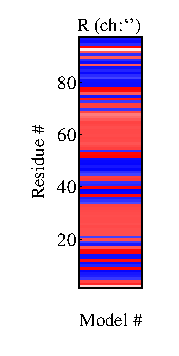
\includegraphics[height=\h\textwidth]{/home/ranjan/Dropbox/ramachandran_number_paper2/git/plotmap/example_pdbs/reports/class_c_a_plus_b_2ACY_chain_.rcode}
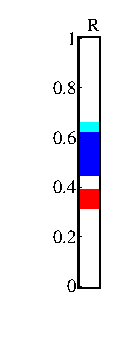
\includegraphics[height=\hc\textwidth]{/home/ranjan/Dropbox/ramachandran_number_paper2/git/plotmap/example_pdbs/reports/class_c_a_plus_b_2ACY_chain_.rcode.eps.colorbar}
\newline
\noindent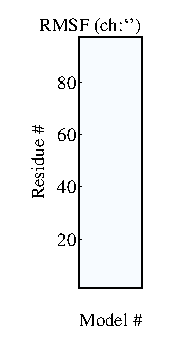
\includegraphics[height=\h\textwidth]{/home/ranjan/Dropbox/ramachandran_number_paper2/git/plotmap/example_pdbs/reports/class_c_a_plus_b_2ACY_chain_.rcode.rmsf}
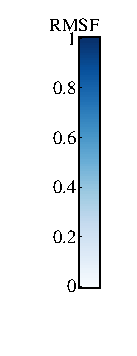
\includegraphics[height=\hc\textwidth]{/home/ranjan/Dropbox/ramachandran_number_paper2/git/plotmap/example_pdbs/reports/class_c_a_plus_b_2ACY_chain_.rcode.rmsf.eps.colorbar}
\newline
\noindent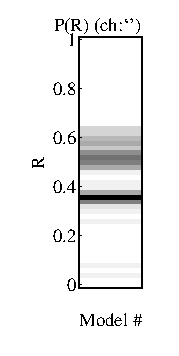
\includegraphics[height=\h\textwidth]{/home/ranjan/Dropbox/ramachandran_number_paper2/git/plotmap/example_pdbs/reports/class_c_a_plus_b_2ACY_chain_.rcode.his}
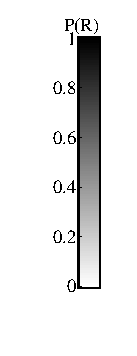
\includegraphics[height=\hc\textwidth]{/home/ranjan/Dropbox/ramachandran_number_paper2/git/plotmap/example_pdbs/reports/class_c_a_plus_b_2ACY_chain_.rcode.his.eps.colorbar}
\newline
\vfill

~

\end{document}